\documentclass{beamer}
\usetheme[compress]{Singapore}

\usepackage{scrextend} % For margins

\usepackage[english]{babel}		
\usepackage[utf8x]{inputenc}
\usepackage{microtype}
\usepackage{graphicx}
\usepackage{amsmath}
\usepackage{amssymb}
\usepackage{amsfonts}
\usepackage{mathtools}
\usepackage{siunitx}
\usepackage{xspace}
\usepackage{mathrsfs}
\usepackage{slashed}
%\usepackage[inline]{enumitem}
\usepackage{enumerate}
\usepackage{cleveref}
\usepackage{booktabs}
\usepackage{bbold}

\usepackage{subcaption}
\usepackage{caption}

\usepackage{animate}

\newcommand{\norm}[1]{\left\lVert#1\right\rVert}
\newcommand{\mb}[1]{\mathbf{#1}}

\title{Structure relaxation using Kernel Ridge Regression}
\author{Malthe Kj\ae r Bisbo}


\begin{document}
\begin{frame}
	\titlepage
\end{frame}

\begin{frame}{ML-enhanced Monte Carlo}
\begin{figure}
	\centering
	\begin{subfigure}{0.5\textwidth}
		\centering
		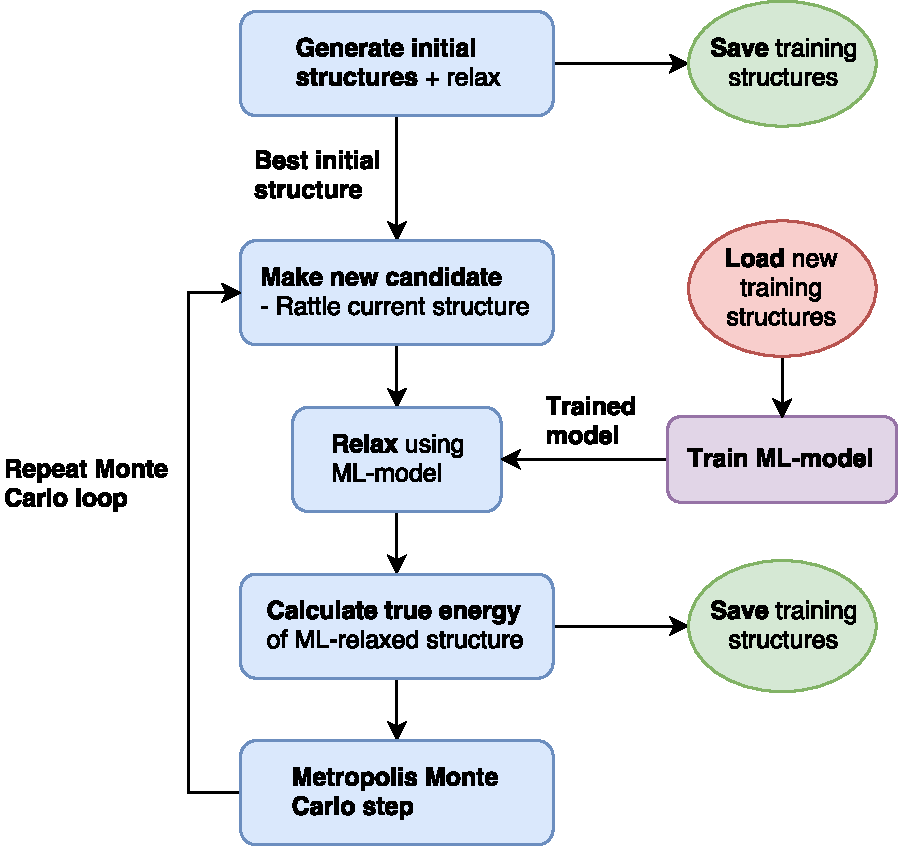
\includegraphics[width=\linewidth]{GlobalSearchModel}
		\caption*{Diagram of the global search method}
	\end{subfigure}%
	\begin{subfigure}{0.5\textwidth}
		\centering
		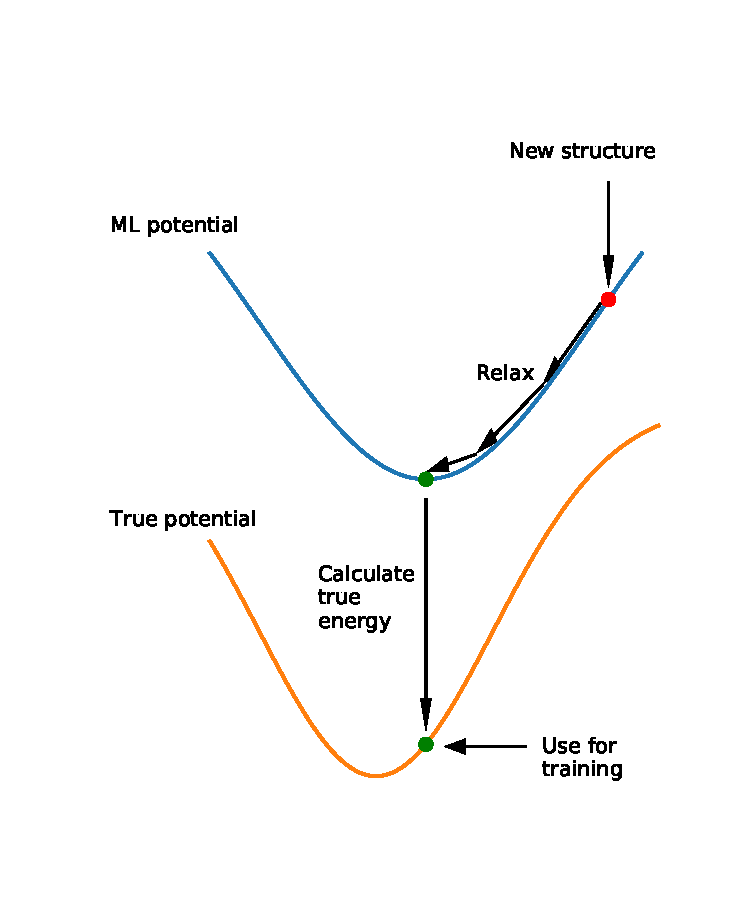
\includegraphics[width=\linewidth]{MLrelaxFigure}
	\end{subfigure}
\end{figure}
\end{frame}

\begin{frame}{KRR/GPR}
	\begin{block}{Prediction}
		\setlength\abovedisplayskip{0pt}
		\begin{flalign*}
		E^*(\mb{x}^*) &= \sum_{i}^{N}\alpha_ik(\mb{x}^*, \mb{x}_i) = \vec{\alpha}^T \vec{\kappa} \\
		F^*(\mb{x}^*) &= -\sum_{i}^{N}\alpha_i \frac{\partial k(\mb{x}^*, \mb{x}_i)}{\partial \mb{r}^*} = -\vec{\alpha}^T \nabla_{\mb{r}^*}\vec{\kappa}
		\end{flalign*}
	\end{block}
	
	\begin{block}{Training}
		\setlength\abovedisplayskip{0pt}
		\begin{flalign*}
		\vec{\alpha} = (\mb{K} + \lambda I)^{-1}\vec{E}
		\end{flalign*}
	\end{block}
	where $k(\cdot,\cdot)$ is the kernel function and $\mb{K}_{ij} = k(\vec{x_i},\vec{x_j})$
\end{frame}

\begin{frame}
	\begin{block}{Gaussian kernel}
	\begin{flalign*}
	k(\cdot,\cdot) = \exp\left(-\frac{d(\cdot,\cdot)^2}{2\sigma^2}\right)
	\end{flalign*}
	with the 2-norm for the dissimilarity d.
	\end{block}
	\begin{block}{Feature}
		\setlength\abovedisplayskip{0pt}
		%For each atomic type combination, the feature is a sum over the gausian-smoothed radial distributions of each atom.
		\begin{flalign*}
		F_{A,B}\left(R\right) = \sum_{A_i, B_j} \frac{\delta\left(R-R_{ij}\right)}{4\pi R^2_{ij}\Delta\left(\frac{N_AN_B}{V}\right)}
		\end{flalign*}
		+ an angular equivalent
	\end{block}
\end{frame}

\begin{frame}{Model system - "Double" Lennard Jones}
	\begin{figure}
		\centering
		\begin{subfigure}{0.5\textwidth}
			\centering
			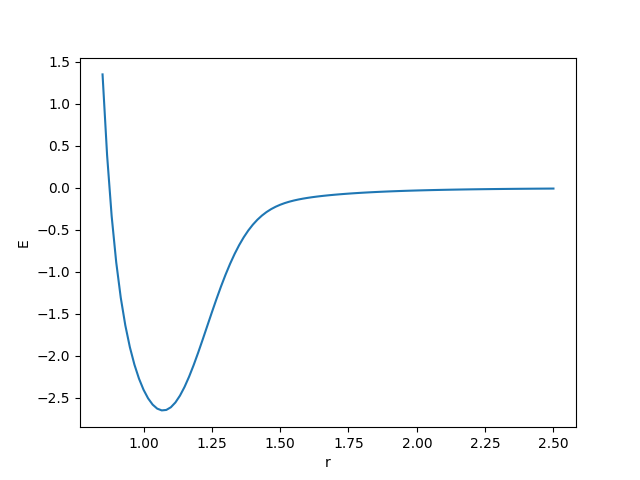
\includegraphics[width=\linewidth]{doubleLJplot}
			\caption*{Interaction potential}
		\end{subfigure}%
		\begin{subfigure}{0.5\textwidth}
			\centering
			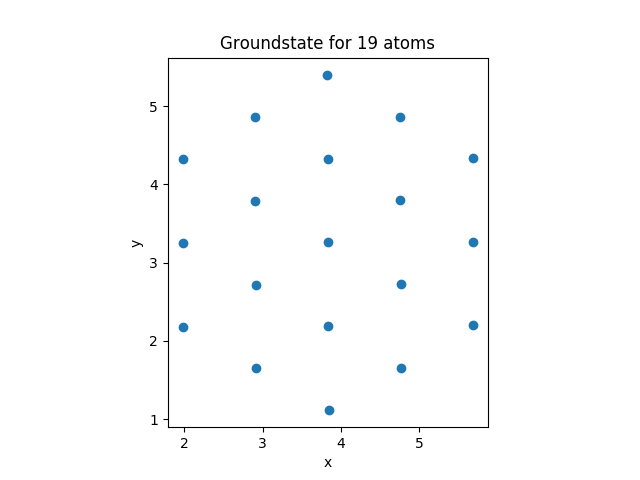
\includegraphics[width=\linewidth]{groundstateStructureN19}
			\caption*{Ground state for 19 atoms}
		\end{subfigure}
	\end{figure}
\end{frame}

\begin{frame}{Search results}
Structures with 19 atoms
\begin{figure}
	\centering
	\begin{subfigure}{0.5\textwidth}
		\centering
		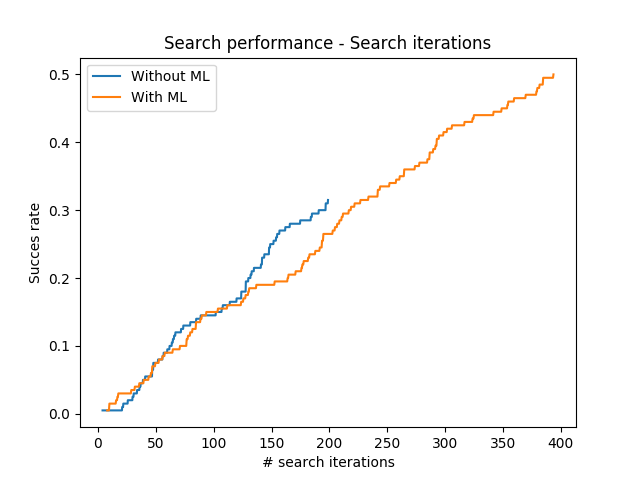
\includegraphics[width=\linewidth]{searchPerform_search_iter}
		\caption*{}
	\end{subfigure}%
	\begin{subfigure}{0.5\textwidth}
		\centering
		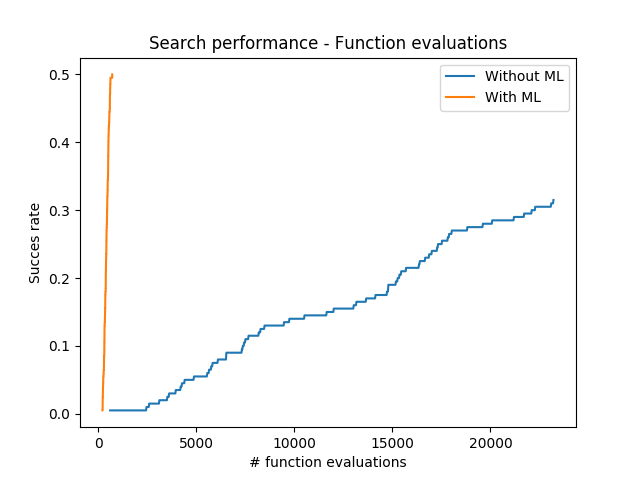
\includegraphics[width=\linewidth]{searchPerform_function_eval}
		\caption*{}
	\end{subfigure}
\end{figure}
\end{frame}

\begin{frame}{Structure check - prediction error}
Filtering unresonable ML-relaxed structures

\bigskip

Rejection criteria:

\centering
\begin{minipage}{0.5\textwidth}
	\begin{align*}
	\text{err}_{KRR} > ..
	\end{align*}
	\begin{figure}
		\centering
		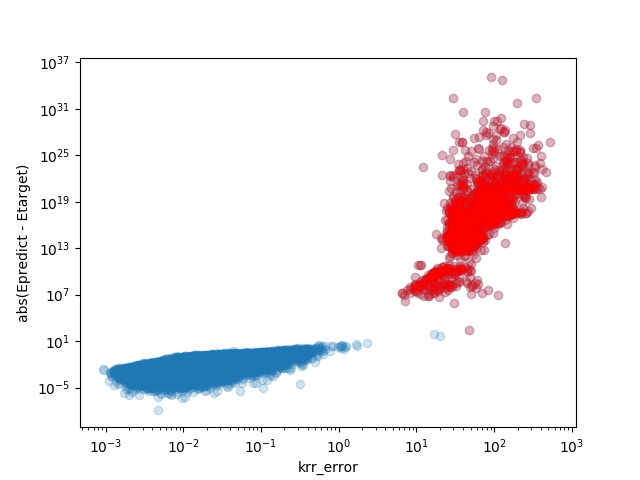
\includegraphics[width=\linewidth, trim={0 0 0 1.5cm}]{error_correlation}
		\caption*{}
	\end{figure}
\end{minipage}%
\begin{minipage}{0.5\textwidth}
	\begin{align*}
	\frac{\text{err}_{KRR}}{\sqrt{\theta_0}} > ..
	\end{align*}
	\begin{figure}
		\centering
		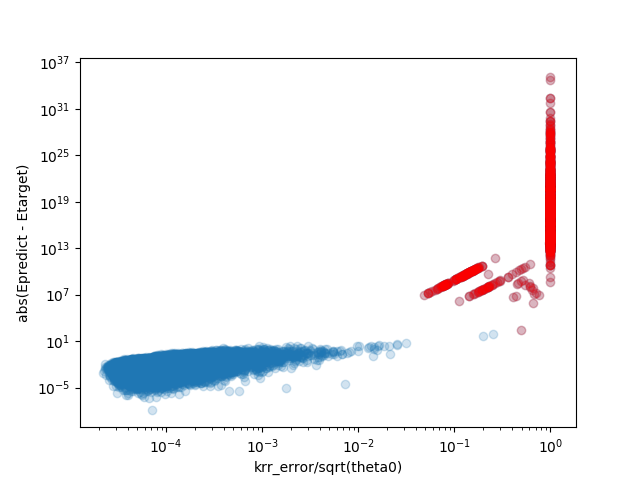
\includegraphics[width=\linewidth, trim={0 0 0 2.2cm}]{error_correlation_theta}
		\caption*{}
	\end{figure}
\end{minipage}
\end{frame}

\begin{frame}{Video demonstration}
	\animategraphics[loop,controls,width=0.4\linewidth]{10}{train_png/train}{0}{20}
\end{frame}


\end{document}